%%%%%%%%%%%%%%%%%%%%%%%%%%%%%%%%%%%%%%%%%%%%%%%%%%%%%%%%%%%%%%%%%%%%%%%%
%    INSTITUTE OF PHYSICS PUBLISHING                                   %
%                                                                      %
%   `Preparing an article for publication in an Institute of Physics   %
%    Publishing journal using LaTeX'                                   %
%                                                                      %
%    LaTeX source code `ioplau2e.tex' used to generate `author         %
%    guidelines', the documentation explaining and demonstrating use   %
%    of the Institute of Physics Publishing LaTeX preprint files       %
	%    `iopart.cls, iopart12.clo and iopart10.clo'.                      %
%                                                                      %
%    `ioplau2e.tex' itself uses LaTeX with `iopart.cls'                %
%                                                                      %
%%%%%%%%%%%%%%%%%%%%%%%%%%%%%%%%%%
%
%
% First we have a character check
%
% ! exclamation mark    " double quote  
% # hash                ` opening quote (grave)
% & ampersand           ' closing quote (acute)
% $ dollar              % percent       
% ( open parenthesis    ) close paren.  
% - hyphen              = equals sign
% | vertical bar        ~ tilde         
% @ at sign             _ underscore
% { open curly brace    } close curly   
% [ open square         ] close square bracket
% + plus sign           ; semi-colon    
% * asterisk            : colon
% < open angle bracket  > close angle   
% , comma               . full stop
% ? question mark       / forward slash 
% \ backslash           ^ circumflex
%
% ABCDEFGHIJKLMNOPQRSTUVWXYZ 
% abcdefghijklmnopqrstuvwxyz 
% 1234567890
%
%%%%%%%%%%%%%%%%%%%%%%%%%%%%%%%%%%%%%%%%%%%%%%%%%%%%%%%%%%%%%%%%%%%
%




\documentclass[12pt]{iopart}
\newcommand{\gguide}{{\it Preparing graphics for IOP Publishing journals}}

%Uncomment next line if AMS fonts required
%\usepackage{iopams}  
\usepackage{amsfonts}
\usepackage{amssymb}
\usepackage{xcolor}
\usepackage{color, colortbl}
\usepackage{pdfpages}
\usepackage{float}
\usepackage{multirow}
\usepackage{multicol}
\usepackage{amsbsy}
\usepackage[none]{hyphenat}
\usepackage{footnote}
\usepackage{tabularx}
\usepackage{epstopdf}
\usepackage{setspace} % for double spacing, maybe remove later
\usepackage{mathrsfs} 
\usepackage[hyphens]{url}
\usepackage[english]{babel}
\usepackage{harvard}
\usepackage{soul}
\usepackage[flushleft]{threeparttable}
\usepackage{changepage}


\makeatletter
\newif\ifnobrackets
\renewcommand\@cite[2]{\ifnobrackets\else[\fi{#1\if@tempswa , #2\fi}\ifnobrackets\else]\fi\nobracketsfalse}
\newcommand\nbcite{\nobracketstrue\cite}
\makeatother
	
\definecolor{Gray}{gray}{0.9}


\begin{document}

% change the following at uni. 24.12.2018
%\pdfminorversion=4
\submitto{\ERL}
\makesavenoteenv{tabular}

\title{The Effects of weather on maize yield: New evidence from Kenya}

\author{Monika Novackova, Martin Todd, Dominic Kniveton and Pedram Rowhani}

\address{Department of Geography, University of Sussex, Falmer, UK}
\ead{monika.novac@gmail.com}
\vspace{10pt}
\begin{indented}
\item[]November 2018
\end{indented}

\doublespacing
\begin{abstract}
...Applying the linear mixed effects models, we found that...\\
\textcolor{blue}{.. to be written later..}
\end{abstract}

%
% Uncomment for keywords
%\vspace{2pc}
%\noindent{\it Keywords}: XXXXXX, YYYYYYYY, ZZZZZZZZZ
%
% Uncomment for Submitted to journal title message
%\submitto{\JPA}
%
% Uncomment if a separate title page is required
%\maketitle
% 
% For two-column output uncomment the next line and choose [10pt] rather than [12pt] in the \documentclass declaration
%\ioptwocol
%
\maketitle
\section{Introduction}\label{Introduction}


\begin{itemize}
\color{blue}
\item[] \textbf{Paragraph 1}

\begin{itemize}

\item Extreme weather causes disasters $\rightarrow$	 early warning systems have been developed
\end{itemize}
\item[] \textbf{Paragraph 2}
\begin{itemize}
\item What weather forecasts (measures) have been used in EWS? \textit{ref. litrature}
\begin{itemize}
\item Mostly seasonal precip. totals and temperature averages
\end{itemize}
\end{itemize}

\item[] \textbf{Paragraph 3} 
\begin{itemize}

\item Identify difference between hazard and disaster

\begin{itemize}
\item Not every hazard turns into disaster
\item For a hazard to become a disaster it needs to have \textbf{impact}
\item Here, we identify the key metrics which have impact on yield
\end{itemize}

\end{itemize}

\item[] \textbf{Paragraph 4}
\begin{itemize}
\item Crop yield versus climate forecasting
\end{itemize}


\item[] \textbf{Paragraph 5}
	\begin{itemize}
		\item Aim of the paper
		\end{itemize}
	 
	\end{itemize}





\section{Methods}\label{Methods}
\color{blue}

...a case study looking at Kenya...
\color{black}


 
\subsection{Data}\label{Data}

In this study, we analysed the relationship between maize yields and climate. Our dataset consisted of an yearly panel of $47$ counties of Kenya describing the period of $1981-2017$. 
	We acquired the county level yearly yield data from the Famine Early Warning Systems Network (FEWS NET). Regarding the weather data, we exploited $0.25^\circ$ resolution precipitation and temperature gridded datasets. The precipitation data were obtained from the Climate Hazards Group InfraRed Precipitation with Station data (CHIRPS) while the temperature data are available at the website of the Berkeley Earth. We calculated spatial averages of the gridded data over the counties to get a single value for each county and each point in time. The frequency of precipitation and temperature data was daily, therefore, further aggregation was needed to obtain yearly values corresponding to the yearly frequency of the yield data. Hence, each weather characteristic was further aggregated over years resulting in a county-level panel conformable with the yield data. 
	
	There are two predominant rainfall regimes in Kenya. The arid and semi-arid (ASAL) counties exhibit mostly bi-modal precipitation patterns with long rains lasting from March to May and short rains occurring between October and December. In the non-ASAL counties, the single rainy season usually starts in March and lasts until August. Following the precipitation patterns and the closely related planting and harvesting calendar, we computed yearly values of various weather characteristics as follows: For the ASAL counties, we used daily data covering October, November and December of the previous year and March, April, May of the current year and for the non-ASAL counties we used daily data covering March to August of the current year.


Following the procedure described above, we calculated a number of previously used characteristics of precipitation and temperature including indicators of floods. These measures are listed in table~\ref{vars} in the appendix. The measures which we found significant were: Total seasonal precipitation and its squared values, average seasonal temperature, coefficient of variation (CV) of seasonal precipitation, CV of average seasonal temperature (converted into Kelvin because the Celsius scale is interval and CV does not have any meaning for data measured on an interval scale),  maximum length of dry spell measured as number of consecutive dry days and the number of dry spells lasting for four days or more (for the purpose of this study we defined a dry day as a day when precipitation didn't exceed $1$mm). We did not include squared values of the average seasonal temperature in our preferred models as it was not significant and most of the past literature has not supported the evidence of the non-linear relationship between yield and temperature.
\subsection{Statistical approach}\label{stats}

% No need to write too many details (or a section) about measures of food security
% No need to describe all the weather measures/characteristics that we have calculated and/or tried to use and didn't work

\sloppy
Kenya consists of $47$ counties with semi-autonomous county governments. As a result of the high degree of county-level autonomy, the policies and regulations often differ across the counties, hence the effects of weather on crop yield are likely to be different across the counties. Therefore, following the standard methodology, we estimated a battery of linear mixed effects models (also known as mixed models) commonly used to analyse longitudinal data \cite{bates2000mixed}. Mixed models are suitable for analysis of panel data as they account for the panel structure of the dataset. These types of models include both fixed effects parameters and random effects. Fixed effects are analogous to parameters in a classical linear regression model and value of each effect is assumed to be fixed over all counties \cite{bates2010lme4}. On the other hand, random effects are unobserved random variables. There are at least three benefits of treating a set of parameters as a random sample from some distribution. \textit{(i)} Extrapolation of inference to a wider population \textit{(ii)} improved accounting for system uncertainty and \textit{(iii)} efficiency of estimation \cite{KERYch9,KERYch12}.

Formally, a linear mixed model can be described by the distribution of two vectors of random variables: the response $\mathscr{Y}$ and the vector of random effects $\mathscr{B}$. The distribution of $\mathscr{B}$ is multivariate normal and the conditional distribution of $\mathscr{Y}$ given $\mathscr{B}=\mathbf{b}$ is multivariate normal of a form %(\citealp{bates2010lme4, KERYch9}):




\begin{equation}\label{MixedGeneral}
\begin{array}{lcl}

(\mathscr{Y}|\mathscr{B}=\mathbf{b})& \sim & \mathit{N}(\mathbf{X}\mathbf{\beta}+\mathbf{Z}\mathbf{b},\sigma^2\mathbf{I}),

\end{array}
\end{equation}

where $\mathbf{X}$ is an $n \times p$ model matrix of fixed effects, $\mathbf{\beta}$ is a $p$-dimensional fixed-effects parameter, $\mathbf{Z}$ is an $n \times q$ model matrix for the $q$-dimensional vector of random-effects variable $\mathscr{B}$ evaluated at $\mathbf{b}$ and $\sigma$ is a scale factor. The distribution of $\mathscr{B}$ can be written as: 

\begin{equation}\label{ranefDist}
\mathscr{B} \sim \mathit{N}(0,\mathbf{\Sigma}),
\end{equation}

where $\mathbf{\Sigma}$ is a $q \times q$ positive semi-definite variance-covariance matrix.





It was apparent from the histogram of the maize yield data that the distribution of maize yield was closer to a log-normal than to a normal distribution. Therefore, we opted for a log-linear functional form of our models as is a common practice in the agricultural economics. Furthermore, we scaled all predictors by subtracting mean and dividing them by standard deviation to avoid convergence problems.


To find the most suitable set of fixed effects, we adapted a stepwise selection procedure which minimized the Akaike's Information Criterion (AIC). The first step of the procedure was the estimation of the model with the complete set of our weather measures in the fixed effects and with the random intercepts. After this, we performed a search through the subsets of the fixed effects minimizing the AIC and allowing for steps in both `backward' and `forward' directions (that is removing and adding the predictors). We decided not to include number of heatwave days and average maximum daily temperature although including them as fixed effects would slightly improve the AIC. The reasons for not including them were their strong correlation with average seasonal temperature (the correlation coefficient was $0.981$ in the case of maximum daily temperature and $0.517$ for the number of heatwave days with the p-values smaller than $1\times10^{-6}$ in both cases), high variance inflation factor (VIF) of the maximum temperature ($5.397$) and the lack of significance of their individual t-tests (the p-values were $0.121$ for the maximum daily temperature and $0.075$ for the number of heatwave days). Furthermore, including heatwave days and maximum daily temperature would only lead to a small change in the AIC from $2080.877$ to $2076.439$ (these values differ from the AIC presented in table~\ref{ARMA} in the appendix because the final estimates reported in table~\ref{ARMA} were estimated using the restricted maximum likelihood (REML) whereas the models were re-estimated using the ML method for comparison\footnote{REML is generally the preferred estimation method for the mixed effects models as the ML estimates of the variance component are biased, however, the REML criterion is not meaningful for comparison of the models with different fixed effects. Therefore, we re-estimated the models by ML for the purpose of comparison \cite{Zuur2009}.}). In addition, the coefficients of both heatwave days and maximum daily temperature were positive, which is opposite to what we expected. Hence, we concluded that the decrease in the AIC and the positive signs are likely to be results of the high correlation with average temperature and we did not include them in our preferred specification.

We further applied a series of likelihood ratio tests to test for the significance of random slopes. No subset of the random slopes improved the fit; therefore, besides the fixed effects, our final model only included the random intercepts.\footnote{Although adding the random slope of CV improved the AIC from $2122.226$ to $2122.110$, we decided to not to include CV of temperature in the random effects. The reason for not including the random slope is that the difference in AIC was negligible and the F-test of the comparison of the two models was insignificant favouring the simpler model (p-value$=0.128$).} 

To verify our results, we adapted an alternative step-down model building
approach using the Satterthwaite’s method to determine the p-values of the individual
t-tests \cite{lmerTest}. We started with a model which included the complete set of our weather measures in both fixed effects and random effects. In the first part of the procedure, the insignificant random effects were removed one by one. In each iteration, the insignificant variable with the highest p-value was removed. This was repeated until only the significant predictors remained. After this, we applied an analogous procedure to the fixed effects until we were left only with the significant variables. As recommended in literature, we considered the level of significance $\alpha=0.1$ for random effects and $\alpha=0.05$~ for fixed effects \cite{lmerTest}. This method led to the same model as the one obtained with our primary AIC-based method described above.


According to the conditional Lagrange multiplier (LM) test developed by Baltagi \& Li (1991) and Baltagi \& Li (1995), the errors exhibited a within group autcorrelation structure in our models (the p-value of the LM test was $1.1\times10^{-13}$). To further investigate the autocorrelation structure of the errors, we estimated a number of models (with the subset of predictors chosen as described above) with an ARMA($p$,$q$) error structure. In particular, we estimated all variants of our model with ARMA($p$,$q$) errors such that $p\leq2$ and $q\leq2$. Comparing the AIC criteria and using the corresponding likelihood ratio statistics, we found that the most appropriate error correlation structure was ARMA($1$,$1$). The value of the AIC criterion of the model with the ARMA($1$,$1$) error structure was $2122.2$ while the AIC was $2129.2$ for the model with ARMA($1$,$0$) errors.  The p-value of the likelihood ratio test of the comparison of the model with ARMA($1$,$1$) errors and the model with ARMA($1$,$0$) errors was smaller than $0.003$, hence the ARMA($1$,$1$) error structure turned out to be a better fit. The AIC criteria and the likelihood ratio tests of all the models with ARMA($p$,$q$) errors are summarised in table~\ref{ARMA} in the appendix.

	\section{Results}\label{Results}
	
Besides our main model, we estimated the same specification for two additional subsamples of the Kenyan counties. In particular, we estimated the model for the subsample of the ASAL counties and for the subsample of the non-ASAL counties separately to compare the effects of various weather characteristics across the two areas with the significantly different climate. The estimates of all three models are summarised in table~\ref{MainEst}. The first two columns represent the model for all counties, the third and fourth columns include estimates for the subsample of the ASAL counties and the last two columns describe the estimates based on the subsample of the non-ASAL counties. All predictors were standardised, therefore the estimates and the corresponding p-values can be interpreted as measures of relative importance. As an additional measure of relative importance we included F-values of the type \textit{III} analysis of variance (ANOVA) in table~\ref{MainEst}. The F-tests were conducted using the marginal rather than the sequential sum of squares. That is, for each variable, the F-test is a test of significance of that part of explained sum of squares which can be contributed to the particular explanatory variable. In other worlds, the F-value is a test statistic of comparison of the preferred model (with all the variables in table~\ref{MainEst}) and the model without the explanatory variable in question but including all other predictors. The main advantage of the type~\textit{III} ANOVA is that the test statistic does not depend on the order in which the effects are entered in the model.

The preferred specification has a log-linear functional form, therefore the estimates in table~\ref{MainEst} are not directly interpretable as marginal effects and their effects are multiplicative. The predicted marginal effects of all coefficients are depicted in figures~\ref{MarEff1} in this section and in figures~\ref{MarEff2} and~\ref{MarEff3} in the appendix. The units of all predictors in all three figures are multiples of their standard deviations since the predictors were standardised. For the values of the marginal effects smaller than one, the effect on yield is negative while marginal effects higher than one can be interpreted as positive effect. The exponents of the estimates (which can be interpreted as the additive marginal effects on yield) can be found in table~\ref{KenARe11_exponents} in the appendix.


In the following few paragraphs, we will discuss the estimates based on the sample of all counties and after that we will focus on the estimates based on the two subsamples.


{
\begin{threeparttable}
\singlespacing
\caption{\textit{\textbf{Mixed  effects model:} \\ Log of maize yield and weather, ARMA(1,1) errors}}
%KEN11dK  KEN11dK_ASAL    KEN11dK_nonASAL % in the file KEN11d_finals2.R in folder RCodes\DecemberNew												
\label{MainEst} 
\begin{footnotesize}
\lineup
\begin{tabular}{@{}lllllll} 
\br 
\vspace{-0.2cm} \\
  \multicolumn{1}{l}{\vspace{0.1cm}\textbf{ }}  &\multicolumn{2}{c}{\textit{\textbf{All counties}}} &\multicolumn{2}{c}{\textit{\textbf{ASAL}}} &\multicolumn{2}{c}{\textit{\textbf{non-ASAL}}}\\
    \multicolumn{1}{l}{\vspace{0.1cm}\textbf{Fixed effects:}}&\textbf{Estimate}&\textbf{F-value\tnote{a}}% anova(KEN11a, type='marginal')
    &\textbf{Estimate}&\textbf{F-value\tnote{a}}&\textbf{Estimate}&\textbf{F-value\tnote{a}}\\
\mr
\\
\vspace{-0.2cm}Intercept&$\m0.259^{***}$&$19.908$&$\m0.241^{*}$&$5.084$&$\m0.342^{**}$&$9.891$\\
  \\ \vspace{-0.2cm}Prec. total&$\m0.078^{*}$&$\05.358$&$\m0.007^{}$&$0.028$&$\m0.244^{***}$&$19.140$\\
  \\
  \vspace{-0.2cm}Prec. total sq.&$-0.028^{*}$&$\04.263$&$\m0.003$&$0.037$&$-0.127^{***}$&$23.384$\\
    \\ \vspace{-0.2cm}Prec. c. of var.&$-0.079^{\bullet}$&$\03.278$&$-0.031$ &$0.237$&$-0.097$&$\02.326$\\
  \\  \vspace{-0.2cm}Dry spell -length\tnote{b}&$-0.067^{*}$&$\04.800$&$-0.181^{**}$&$6.841$&$-0.012$&$\00.164$\\
  \\ \vspace{-0.2cm}Dry spells 	$\geq$ 4 d.&$-0.063^{*}$&$\04.848$&$-0.156^{**}$&$8.032$&$-0.011$&$\00.087$\\
  \\ \vspace{-0.2cm}Temp. - average&$-0.199^{***}$&$12.010$&$-0.214^{*}$&$5.409$&$-0.128$&$\01.525$\\
  \\  \vspace{-0.2cm}Temp. c. of var.&$\m0.042^{\bullet}$&$\02.961$&$\m0.032$&$0.355$&$\m0.058^{*}$&$\05.372$\\
  \\
  \hline
\vspace{-0.2cm} \\
  \multicolumn{1}{l}{\textbf{Random effects:}}  & \\
\vspace{-0.2cm}
\\
\hline
\\
  \vspace{-0.2cm}Intercept\\
 \\ 
 \hline
\vspace{-0.2cm} \\
\textit{Number of observations:}  &\multicolumn{2}{c}{$1300$}&\multicolumn{2}{c}{$698$}&\multicolumn{2}{c}{$602$}\\
\vspace{-0.2cm}
\\  
\br
\end{tabular} 
\end{footnotesize}
 \begin{tablenotes}
  \begin{footnotesize}
    \item \textit{Notes:} Standard errors in brackets; \hfill $^{\bullet}~p<0.1$; $^{*}~p<0.05$; $^{**}~p<0.01$; $^{***}~p<0.001$
        \begin{adjustwidth}{1cm}{} 
    \item[a] Marginal (type III) sum of squares. The F-statistics correspond to the sum of squares attributable to each fixed effect.
  \item[b] In number of days.
     \end{adjustwidth}
\singlespacing
  \end{footnotesize}
\end{tablenotes}
  \end{threeparttable} 
\par}
\linespread{1}


The estimates of the model of the whole sample are summarised in the first two columns of table~\ref{MainEst}. Consistently with our assumptions, seasonal precipitation and average temperature have significant effects on yield. As we expected, the effect of temperature is negative. The linear term of precipitation is positive while the squared term of precipitation is negative and as we can see in figure~\ref{MarEff1}(a), the plot of the marginal effects of precipitation is hill-shaped. That is, the effect of precipitation is negative and increasing if the amount of precipitation is below its mean and the marginal effect increases with the amount of precipitation until it reaches $1.403$ times its standard deviation. At this point, the effect starts to decrease with increasing precipitation and it becomes negative again once the amount of precipitation reaches $2.805$ times its standard deviation. Therefore, too  much rain is harmful for agricultural yield as well as not enough rain. This is intuitive as extreme rainfall can cause flooding which is damaging for yield.



Besides total cumulative seasonal precipitation and average temperature, CV of both temperature and precipitation and the length and number of dry spells turned out to be significant (see the first column of table~\ref{MainEst}). The relationship of maize yield and each of these variables is linear as is apparent from the figures~\ref{MarEff2}(a) and \ref{MarEff2}(b) in the appendix. In accordance with our expectation, the yield decreases with increasing CV of precipitation. \hl{However, the result for CV of temperature is a bit peculiar as the yield seem to increase with increasing variability of temperature. This is probably because...}
As it is apparent from figures~\ref{MarEff3}(a) and \ref{MarEff3}(b) in the appendix, yield declines with increasing number of dry spells and with length of maximum dry spell linearly. This is in accordance with our expectations.

According to both magnitude of the standardised coefficients and F-values in the first two columns of table~\ref{MainEst}, the most important variable of the model for all counties is average seasonal temperature. Average seasonal temperature has the lowest p-value of the predictors in this model and based on its magnitude and F-value it is much  more important than the second most important variable, which is precipitation.

We will now discuss and compare the results of the models for the subsamples of the ASAL counties (the third and fourth columns of table~\ref{MainEst}) and the non-ASAL counties (the third and fourth columns of table~\ref{MainEst}).



  \begin{figure}% new plots checked and good 17.dec.2018
   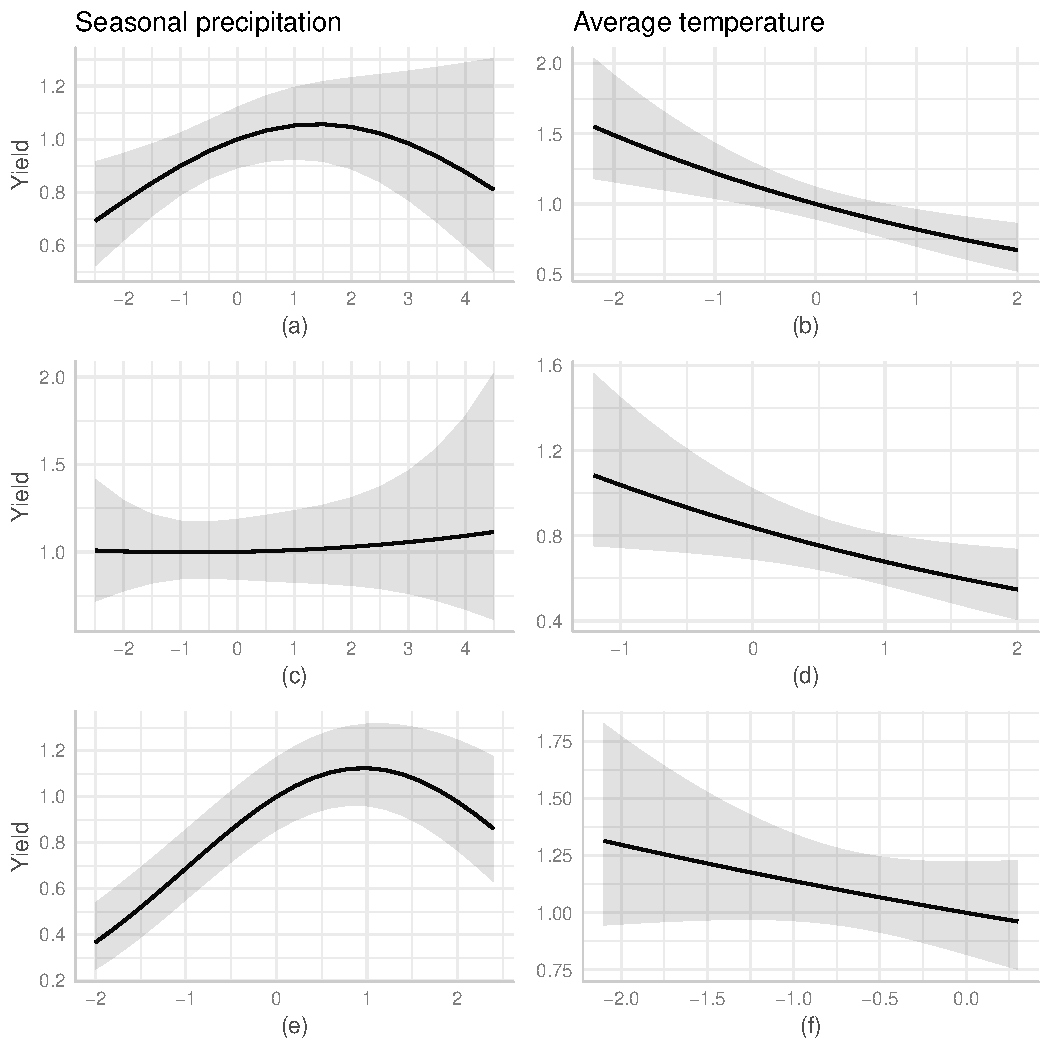
\includegraphics{Figure1a_1f.pdf}
\caption{Predicted multiplicative marginal effects of seasonal precipitation (left column) and average seasonal temperature (right column) on maize yield assuming that all other variables are fixed at their means (which is zero, as the predictors were standardised). The first row (a, b) represents the model for all counties, the second row (c, d) is based on the subsample of arid and semi-arid counties (ASAL) and the third row (e, f) represents the model for the non-ASAL counties. Precipitation and temperature (x-axis) are in multiples of their standard deviations as the models were standardised. The effects are multiplicative as the models are in the log-linear form.}\label{MarEff1}
\end{figure}




\begin{itemize}
\color{blue}
\item Verbal description and interpretation of the results. Discussing goodness of fit using various criteria such as AIC or alternatives to $R^2$.

\item relative importance of the individual variables and its measures
%\item Possibly estimate simple regressions with the same explanatory variables as the preferred mixed effects specification. This would give us an approximation of $R^2$ which could be used to compare our models.

	%	\begin{itemize}%
		%	\item \textcolor{red}{Annemie has advised me that for a more precise approximation of $R^2$ we can estimate a simple regression of yields on the random intercepts (county level dummy variables) and then subtract the $R^2$ of this model from the $R^2$ of the simple regression with the explanatory variables of the preferred mixed models (the model described in the bullet point above). This would give us a percentage of yield variability explained by the weather measures not including the variability explained by the random intercepts.}
	%\end{itemize}
	
	
\item show VIF
\item If we get the yield data for the period from $2015$ onwards: Out of sample predictions and comparison with the real data
\end{itemize}





\color{black}

\clearpage

\appendix
\section*{Appendix}

\textcolor{blue}{\textit{should be at the end of the main text but before list of references}}



\begin{table}[H]
\caption{\label{ASAL}\textbf{List of arid and semi-arid (ASAL) and non-ASAL counties}}

\begin{indented}
\item[]\begin{tabular}{@{}lp{10cm}}
\\[-1em]
\br
\\[-1em]
\textbf{ASAL:}&Baringo, Embu, Garissa, Isiolo, Kajiado, Kilifi Kitui, Kwale, Laikipia, Lamu, Makueni, Mandera, Marsabit, Meru, Mombasa, Narok, Nyeri, Samburu, Taita-Taveta, Tana River, Tharaka Nithi, Turkana, Wajir, West Pokot\\
\mr
\textbf{non-ASAL:}&Bomet, Bungoma, Busia, Elgeyo Marakwet, Homa Bay, Kakamega, Kericho         Kiambu, Kirinyaga, Kisii, Kisumu, Machakos, Migori, Murang'a, Nakuru, Nyamira,   Nyandarua, Siaya, Trans Nzoia, Uasin Gishu, Vihiga\\
\br
\end{tabular}
\end{indented}
\end{table}





\begin{threeparttable}[H]
\singlespacing
\caption{Precipitation and temperature measures considered}\label{vars}
\begin{tabular}{@{}lp{15cm}}
\\[-1em]
\br
\\[-1em]
$\bullet$& Total rainfall over the rainy season\\
$\bullet$& Coefficient of variation of the rainfall during the rainy season\\
$\bullet$& Maximum length of dry spell during the rainy season (in number of days)\\
$\bullet$& Number of dry spells during the rainy season: a dry spell defined as $4$ consecutive days without rain or more\tnote{a}\\
$\bullet$& Number of dry spells during the rainy season: a dry spell defined as $10$ consecutive days without rain or more\tnote{a}\\
$\bullet$& Number of dry spells during the rainy season: a dry spell defined as $20$ consecutive days without rain or more\tnote{a}\\
$\bullet$& Average temperature during the rainy season\\
$\bullet$& Standard deviation of temperature during the rainy season\\
$\bullet$& Cumulative degree days during the rainy season (excluding the days when maximum temperature above $30^{\circ}$C or below $10^{\circ}$C\\
$\bullet$& Number of heatwave days during the rainy season when max. temperature $>35^{\circ}$C
\\
$\bullet$& Maximum daily rainfall  - to control for possible floods
\\
$\bullet$& Sum of precipitation amount on days where precipitation is above $90^{th}$ percentile of precip. of the whole period\tnote{b}\\
$\bullet$& Sum of precipitation amount on days where precipitation is above $95^{th}$ percentile of precip. of the whole period\tnote{c}\\
$\bullet$& Sum of precipitation amount on days where precipitation is above $99^{th}$ percentile of precip. of the whole period\tnote{d}\\
$\bullet$& Number of days where precipitation is above $90^{th}$ percentile of precip. of the whole period\tnote{b}\\
$\bullet$& Number of days where precipitation is above $95^{th}$ percentile of precip. of the whole period\tnote{c}\\
$\bullet$& Number of days where precipitation is above $99^{th}$ percentile of precip. of the whole period\tnote{d}\\
\br
\end{tabular}
\begin{tablenotes}
  \begin{footnotesize}
  \item[a] Threshold for a dry day was considered $1$mm.
  \item[b] $90^{th}$ percentile was calculated for the subsample of wet days, that is the days where precipitation is above or equal to $1$mm.
\item[c] $95^{th}$ percentile was calculated for the subsample of wet days, that is the days where precipitation is above or equal to $1$mm.
  \item[d] $99^{th}$ percentile was calculated for the subsample of wet days, that is the days where precipitation is above or equal to $1$mm.
  \end{footnotesize}
\end{tablenotes}
\end{threeparttable} 




{\begin{center}
\begin{threeparttable}[H]
\caption{\label{ARMA}Comparison of models with different error autcorrelation structure}
\lineup
\begin{indented}

\item[]\begin{tabular}{@{}llll}
\\[-1em]
\br
&&\centre{2}{\textbf{Likelihood ratio} vs. ARMA($1$,$1$)\tnote{a}}\\
\textbf{Error autocorrelation structure}&\textbf{AIC}&\textbf{Statistic}&\multicolumn{1}{l}{\textbf{p-value}}\\
\mr
\textit{None}&$2205.4$&$87.17$&$<1\times10^{-4}$\\
ARMA($1$,$0$)&$2129.2$&$\08.99$&$0.0027$\\
ARMA($0$,$1$)&$2145.0$&${24.73}$&${<1\times10^{-4}}$ \\
\rowcolor{Gray}ARMA(${1}$,${1}$)&${2122.2}$&$---$&$---$\\
ARMA($2$,$1$)&$2124.1$&$\00.15$&$\0\00.6990$\\
ARMA($1$,$2$)& $2124.2$&$\00.01$&$\0\00.9181$\\
ARMA($2$,$2$)&$2125.9$& $\00.31$&$\0\00.8549$\\
\br
\end{tabular}

\end{indented}
\begin{tablenotes}
  \begin{footnotesize}
  \item[a] Likelihood ratio test of a comparison of the model in each row against the ARMA(${1}$,${1}$) error structure model. ARMA(${1}$,${1}$) error structure seems to be the most suitable as all lower-order correlation structure models are rejected against ARMA(${1}$,${1}$) while ARMA(${1}$,${1}$) is not rejected against any of the higher order structures.
\singlespacing
  \end{footnotesize}
\end{tablenotes}
  \end{threeparttable} 
\end{center}


\vspace{1cm}
\textcolor{blue}{Possibly include a table of all values which I get from the lme or lme4 models summary in R, that is. correlation of the fixed effects etcetera}


\textcolor{blue}{Maybe also a table with standard errors here}




{\begin{threeparttable}
\normalsize
\caption{\normalsize{\textbf{ {Mixed  effects model:}} exponents of the coefficient estimates Log of maize yield and weather, ARMA(1,1) errors}}
%KEN11dK  KEN11dK_ASAL    KEN11dK_nonASAL										
\label{KenARe11_exponents} 
\lineup
\begin{tabular}{@{}lllllll} 
\br \\
  \textbf{Fixed effects:}&\textit{\textbf{All counties}}&\textit{\textbf{ASAL}}&\textit{\textbf{non-ASAL}}\\
\mr
\\
\vspace{-0.2cm}Intercept&$1.296^{***}$&$1.272^{*}$&$1.408^{**}$\\
  \\ \vspace{-0.2cm}Prec. total&$1.081^{*}$&$1.007^{}$&$1.277^{***}$\\
  \\
  \vspace{-0.2cm}Prec. total sq.&$0.973^{*}$&$1.003$&$0.881^{***}$\\
    \\ \vspace{-0.2cm}Prec. c. of var.&$0.924^{\bullet}$&$0.970$ &$0.907^{}$\\
  \\  \vspace{-0.2cm}Dry spell -length&$0.935^{*}$&$0.834^{**}$&$ 0.988^{}$\\
  \\ \vspace{-0.2cm}Dry spells 	$\geq$ 4 d.&$0.939^{*}$&$0.855^{**}$&$0.989^{}$\\
  \\ \vspace{-0.2cm}Temp. - average&$0.820^{***}$&$0.808^{*}$&$0.880$ $^{}$\\
  \\  \vspace{-0.2cm}Temp. c. of var.&$1.043^{\bullet}$&$1.032$&$1.060$ ${*}$\\
  \\
  \hline\\[-1em]
  \multicolumn{1}{l}{\textbf{Random effects:}}  & \\ 
  \\[-1em]
\hline
\\[-1em]Intercept\\
 \\[-1em] \hline
\\[-1em]
\textit{Number of observations:}  &\multicolumn{2}{c}{$1300$}&\multicolumn{2}{c}{$698$}&\multicolumn{2}{c}{$602$}
\\
\br
\end{tabular} 
 \begin{tablenotes}
  \begin{footnotesize}
    \item \textit{Notes:} Standard errors in brackets; \hfill $^{\bullet}~p<0.1$; $^{*}~p<0.05$; $^{**}~p<0.01$; $^{***}~p<0.001$
\singlespacing
  \end{footnotesize}
\end{tablenotes}
  \end{threeparttable} 
\par}

\clearpage


  \begin{figure}
   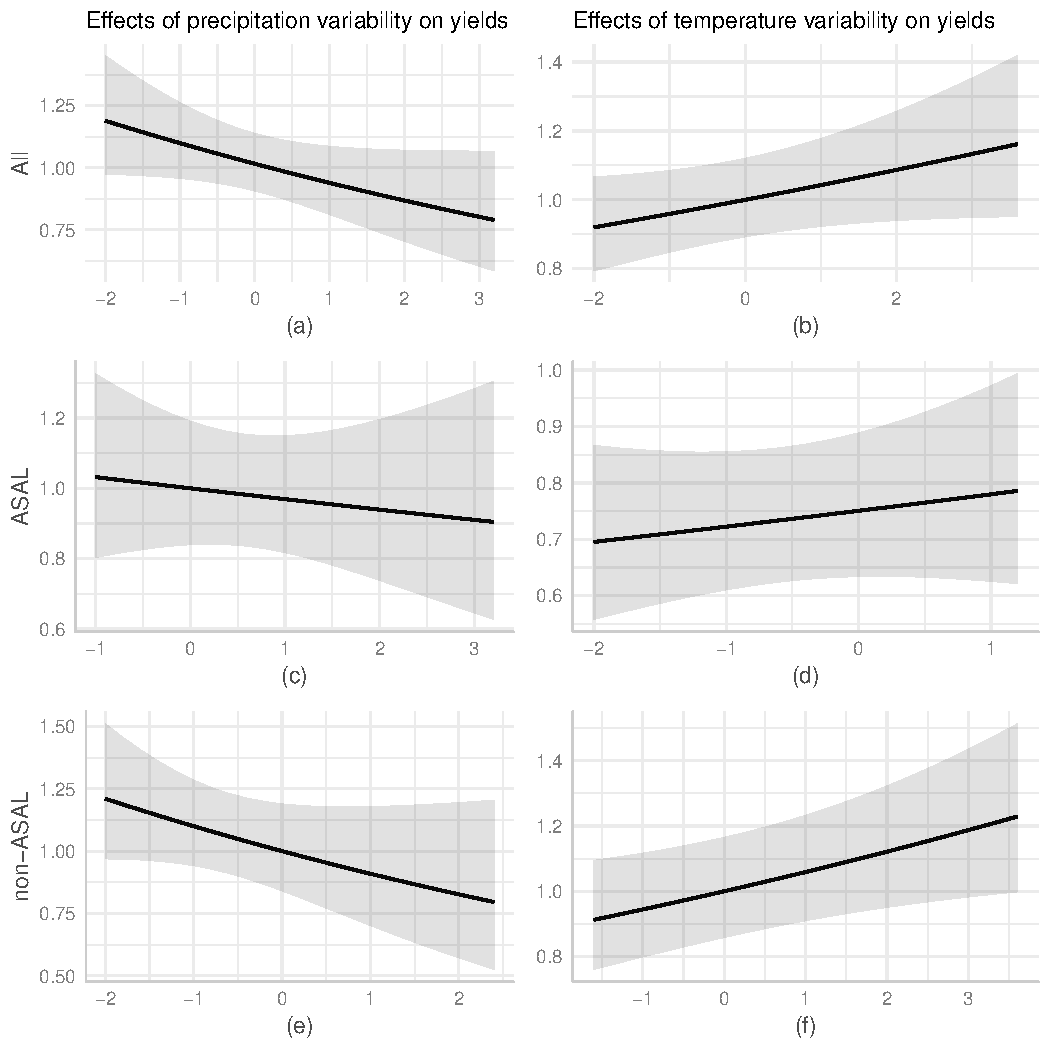
\includegraphics{Figure2a_2f.pdf}
\caption{Predicted multiplicative marginal effects of coefficient of variation (CV) of precipitation (left column) and CV of temperature (right column) on maize yield assuming that all other variables are fixed at their means (which is zero, as the predictors were standardised). The first row (a, b) represents the model for all counties, the second row (c, d) is based on the subsample of arid and semi-arid counties (ASAL) and the third row (e, f) represents the model for the non-ASAL counties. CV of precipitation and temperature (x-axis) are in multiples of their standard deviations as the models were standardised. The effects are multiplicative because the models are in the log-linear form.}\label{MarEff2}
\end{figure}

  \begin{figure}
   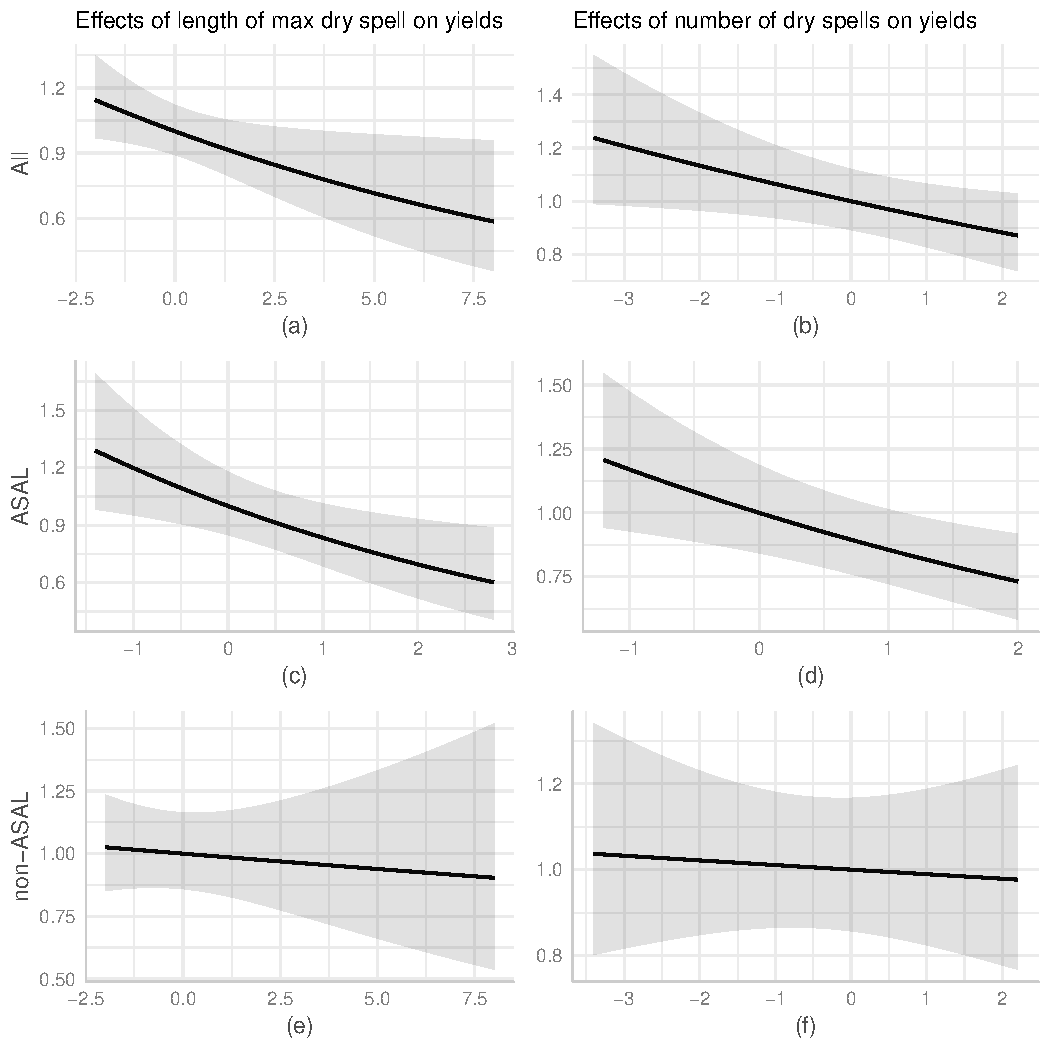
\includegraphics{Figure3a_3f.pdf}
\caption{Predicted multiplicative marginal effects of length of maximum dry spell in days (left column) and number of dry spells lasting for four days or more (right column) on maize yield assuming that all other variables are fixed at their means (which is zero, as the predictors were standardised). The first row (a, b) represents the model for all counties, the second row (c, d) is based on the subsample of arid and semi-arid counties (ASAL) and the third row (e, f) represents the model for the non-ASAL counties. Maximum length of dry spell and number of dry spells (x-axis) are in multiples of their standard deviations as the models were standardised. The effects are multiplicative because the models are in the log-linear form.}\label{MarEff3}
\end{figure}


\section*{References}



\bibliography{referencesFS}

\bibliographystyle{dcuM}
\nocite{Baltagi91}
\nocite{Baltagi95}
\nocite{ASF} 
\nocite{Berkeley} 
\nocite{CHIRPS} 
\nocite{FEWSNET}

\end{document}

